\documentclass[a4paper]{article}
\usepackage{amsmath}
\usepackage{amsfonts}
\usepackage{amssymb}
\usepackage{graphicx}
\usepackage{booktabs} 
\usepackage{hyperref}
\usepackage{geometry}
\usepackage{caption}
\usepackage{float}

\begin{document}

\begin{titlepage}
    \vspace*{2cm}
    \begin{center}


    \begin{figure}
    \centering
        
\includegraphics[width=0.6\linewidth]{unilogo.png}
    \end{figure}

    \vspace*{2cm}

    \LARGE

    \textbf{LLM Benchmark project Report}


    \vspace{3.5cm}
    \normalsize
    \begin{minipage}[t]{0.47\textwidth} 
        {Professors:} \vspace{0.3em} \\
        {\large \textbf{Michele Lombardi}} \vspace{1em}\\
        {\large \textbf{Allegra De Filippo}}
    \end{minipage}
    \hfill
    \begin{minipage}[t]{0.47\textwidth}\raggedleft
    {Students:} \hspace{-0.9em} \vspace{0.3em} \\
        {\large \textbf{Simone Migliaccio (matr.: 0001159303)}}\vspace{0.2em}\\
        {\large \textbf{Simone Spezia (matr.: 0001167605)}}\vspace{0.2em}\\
        {\large \textbf{Alberto Varini (matr.: 0001189363)}}\\
    \end{minipage}

    \end{center}

\end{titlepage}

\newpage


\section{Introduction}
The main goal of this project is to provide a general benchmark to evaluate different LLMs performances under different types of planning domains to better understand in advance what are the planning capabilities of a given LLM. In the following sections the main features of this projects are going to be shown.

\section{PDDL Problems Classification}
The first thing to do since we wanted a trustable benchmark and since a lot of PDDL models were already provided as reference material was to classify the problems 
using a numerical difficulty score. We used a numerical score because it is intuitively understandable by anyone who will ever want to compare the performance of 
LLMs using these models.
Another classification implemented consists into separating problems in different categories based on the type of reasoning they request.
To compute the scores the code can be found in the file \texttt{score\_domains\_complexity.py}

    \subsection{Difficulty Classification}
    \subsubsection{Instances scores}
    The complexity of a single problem instance is calculated using a weighted logarithmic combination of four key metrics. The use of the logarithm prevents any single feature from dominating the score excessively.\\

    The \textbf{Raw Score} is defined as:
    \begin{equation}
        Raw\_score = 0.45 \cdot \log(1 + A) + 0.20 \cdot \log(1 + G) + 0.20 \cdot \log(1 + N) + 0.15 \cdot T
    \end{equation}

    Where:
    \begin{itemize}
        \item \textbf{A (Actions):} Number of feasible grounded actions. This is estimated by unifying action parameters with objects that satisfy static preconditions in the initial state.
        \item \textbf{G (Goals):} Total number of atomic conditions in the goal state.
        \item \textbf{N (Numeric Score):} A composite value representing numeric complexity:
        \begin{equation}
            N = E_{num} + 2 \cdot P_{num} + 3 \cdot G_{num} + M
        \end{equation}
        where $E_{num}$ are numeric effects, $P_{num}$ numeric preconditions, $G_{num}$ numeric goal conditions, and $M$ is a binary flag for the presence of a metric.
        \item \textbf{T (Topology Score):} Evaluates the spatial/relational complexity based on predicates like \textit{adj} or \textit{connected}:
        \begin{equation}
            T = \log(1 + Nodes) + \log(1 + Edges) + Density
        \end{equation}
    \end{itemize}
    Obviously a different weight could be assigned to each different part of the computation of raw scores depending on the operator that is doing the tests in order to higlight more for example the number of action present in the instances and so on.\\
    Finally, an \textbf{Instance Score (0-100)} is calculated by normalizing the raw score relative to the minimum and maximum scores found within the same domain. The results can be found in the folder \texttt{domains\_complexity}.\\
    Note that also some additional statistics for each domain are computed based on the results obtained from the instances, for example it could be of interest evaluating the mean and the median of the scores obtain form the instances of a single domain.

    \subsubsection{Domain scores}
    The overall difficulty of a domain is not just the average of its instances, but a reflection of its total state-space and constraint complexity.
    The \textbf{Domain Difficulty (0-100)} is computed by:
    \begin{enumerate}
        \item Summing the $S_{raw}$ of all instances belonging to the domain to obtain a \textit{Total Raw Score}.
        \item Normalizing this total across all tested domains in the benchmark.
    \end{enumerate}
    This approach ensures that a domain with many complex instances is ranked higher than one with few simple instances, note that obviously the easiest problems gets a domain difficulty equal to 0 (in this case is the "fo-sailing" problem) and the problem with the highest difficulty has domain difficulty equal to 100, (in our case the "settlersnumeric" problem).

    \subsubsection{Results obtained}
    In order to obtain a visual representation of the classified problems, we produced heatmaps for both the overall normalized domain scores and the raw scores.
    \begin{figure}[H]
    \centering
        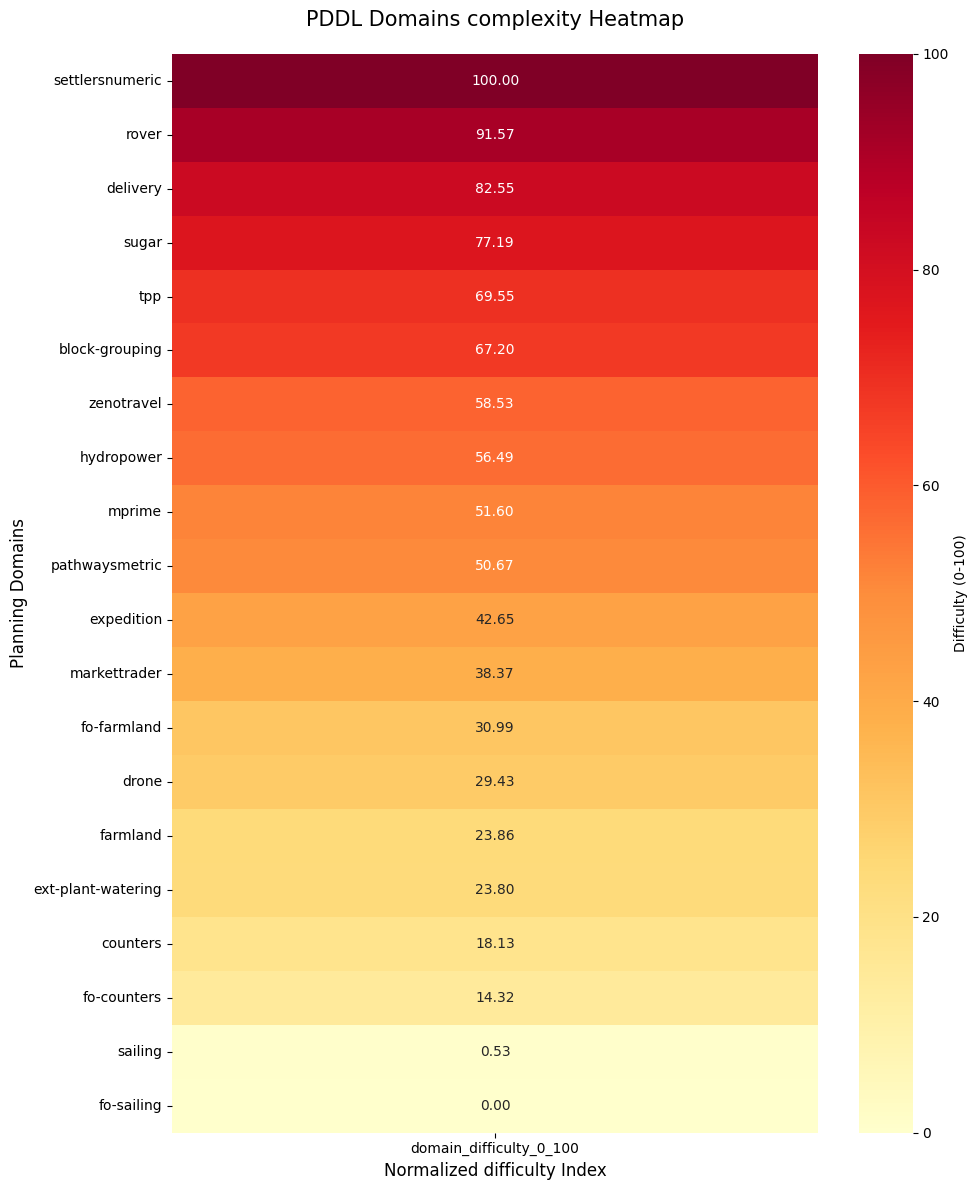
\includegraphics[width=0.6\linewidth]{domaincompl.png}
    \end{figure}

    \begin{figure}[H]
    \centering
        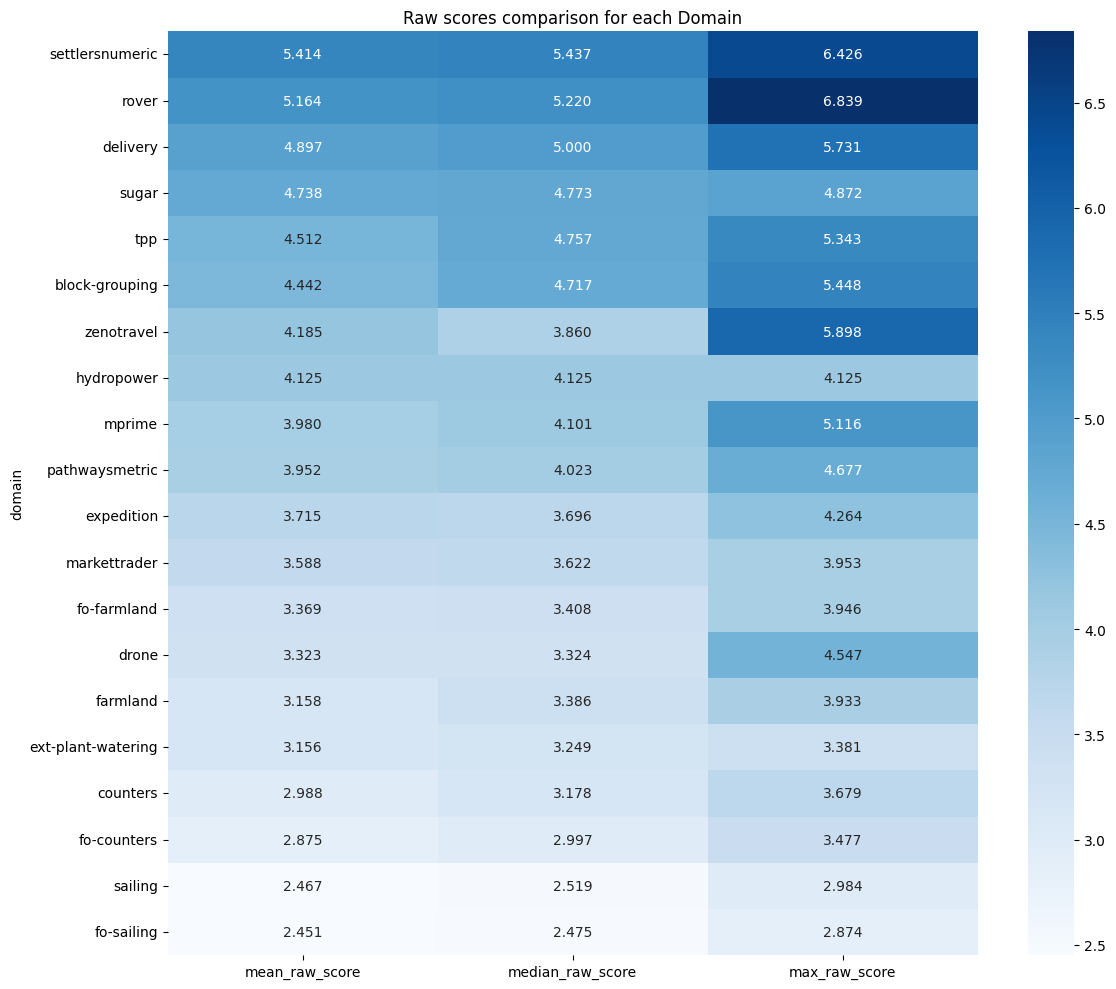
\includegraphics[width=0.6\linewidth]{rawscoreshm.png}
    \end{figure}

    
    \subsection{Reasoning Classification}
    Here the classification based on the type of reasoning these problems require the LLM to employ is shown. We decided to split the reasoning types into 5 categories:
    \begin{itemize}
        \item \textbf{Spatial:} These problems are typically about objects that have to be moved in a 2D (or more dimensional) spaceframe.
        \item \textbf{Numerical Optimization:} These problems require from the LLM an extensive capacity to deal with numerical optimization problems, such as managing complex cost functions and resource constraints.
        \item \textbf{Temporal Planning:} In this kind of problem it is required from the LLM to be able to reach the goal defining an order between objects having timing constraints and relations.
        \item \textbf{Logistic:} In this kind of problems it is required to reach the goal by planning some kind of goods transportation and agents coordination.
        \item \textbf{Logic:} These are abstract puzzles where the state space and actions represent symbolic or mathematical transformations rather than physical interactions. They test the model's ability to reason over purely formal rules without relying on world knowledge.
    \end{itemize}

    In the following table the classification of the 20 planning problems is shown, note that in this case all the work have been done by hand and that the problems in the table are ordered form hardest to easiest following the previous difficulty classification.
    
    \begin{table}[H]
        \centering
        \renewcommand{\arraystretch}{1.25} 
        
        \begin{tabular}{c|c}
            \toprule
            
            \textbf{PDDL Problem} & \textbf{Reasoning Category} \\
            
            \midrule[1pt]
            \addlinespace[0.25cm]
            Settlersnumeric & Numerical Optimization \\
            \midrule
            Rover & Logistic \\
            \midrule
            Delivery & Logistic \\
            \midrule
            Sugar & Numerical Optimization \\
            \midrule
            Tpp & Numerical Optimization \\
            \midrule
            Block-Grouping & Spatial \\
            \midrule
            Zenotravel & Logistic \\
            \midrule
            Hydropower & Temporal Planning \\
            \midrule
            Mprime & Logic \\
            \midrule
            Pathwaysmetric & Numerical Optimization \\
            \midrule
            Expedition & Logistic \\
            \midrule
            Markettrader & Numerical Optimization \\
            \midrule
            Fo-farmland & Numericaal Optimization \\
            \midrule
            Drone & Spatial \\
            \midrule
            Farmland & Numerical Optimization \\
            \midrule
            Ext-Plant-Watering & Spatial \\
            \midrule
            Counters & Numerical Optimization \\
            \midrule
            Fo-Counters & Numerical Optimization \\
            \midrule
            Sailing & Spatial \\
            \midrule
            Fo-Sailing & Spatial \\
            
        \end{tabular}
        \vspace{0.2cm}
        \caption{Risultati di classificazione per le 20 istanze, con parametri centrati.}
        \label{tab:dati_pfile_griglia}
    \end{table}




    \subsection{Problems chosen}

    % inserire che problemi sono stati scelti per essere dati agli LLM
    By combining instance-level and domain-level metrics, we can categorize problems into three tiers: \textbf{Easy}, \textbf{Medium}, and \textbf{Hard}. This classification is fundamental to evaluate if an LLM's success rate drops predictably as the complexity of the grounded action space or numeric constraints increases.


\section{Parser and LLMs Models Implemented}


\section{Validator}


\section{Output Comparison}


\section{Risultati}
% Esempio di come potresti strutturare una tabella per i risultati
\begin{table}[h]
    \centering
    \caption{Performance dei modelli nel dominio Farmland}
    \begin{tabular}{lccc}
        \toprule
        Modello & Success Rate (\%) & Lunghezza Media Piano & Iterazioni Medie \\
        \midrule
        GPT-4o & 85.0 & 12.4 & 1.2 \\
        Gemini 1.5 Pro & 88.5 & 11.8 & 1.1 \\
        Llama 3 70B & 72.0 & 14.2 & 2.4 \\
        \bottomrule
    \end{tabular}
\end{table}

\section{Conclusioni}
Discussione finale sui risultati ottenuti e suggerimenti per future estensioni del benchmark, come l'aggiunta di domini temporali.

\bibliographystyle{plain}
% \bibliography{references} % Se hai un file .bib

\end{document}